\section{Stocks}

\indent \newline
The existing simulation model is expanded through adding new stocks and flows, as well as the relations from the causal loop diagram. The expanded model consists of the most important variables, when it comes to improving waste sorting behavior and the material recycling rate. The added stocks results in a better understanding of how these variables can be influenced. Some of the variables from the causal loop diagram were changed into stocks based on these criteria:

\indent \newline
\begin{enumerate}
\item The units of measure are usually a quantity, and difficult to change in a moment.
\item Should give the system inertia.
\item	If the variable represents a behavior which is important in the dynamics we want to explain. 
\cite[p. 192]{system}
\end{enumerate}


\indent \newline
The following variables were converted directly into stocks; household knowledge, advertising and improvements to waste management system. These are in turn influenced by other variables and causal links from the causal loop model. Primarily, the variable household knowledge was added directly into the model as a stock. Studies show that household knowledge leads to a better attitude towards waste sorting, which will have a positive effect on waste sorting behavior \cite[p. 13, Preliminary report]{intention}.The variable "improvements to waste management system" from the causal loop diagram was converted into the stock "waste management system in practice". The stock represents improvements and changes made to the waste management system. The model accumulates the change in the system over time. Lastly, the stock "advertising effectiveness in practice" was added in order to measure the effect on attitude. 

\section{Values}

\indent \newline
The original waste supply chain model was designed for simulating the material recycling rate for the total population. Since this paper focuses on 20-39 year old's, not coming from Asia, Africa, Latin-America and Eastern Europe outside of EU, it has been necessary to make some adjustments. For the model to represent the intended target group, values have been changed in some of the variable’s associated equations.

\indent \newline
The following variables have been tweaked: "paper in households 2018", "food in households 2018", "plastic in households 2018", "rest waste in households 2018", "other energy inflows" and "other material inflows". All of the mentioned variable's initial values have been multiplied with 0.27, because the target group represents 27\% of Oslo's population. 

\section{Main Systems}

\indent \newline
By adding the variables from the causal loop diagram, the stock and
flow model increases in complexity. Because of this, the model is split 
into eight main systems: 

\indent \newline
\begin{enumerate}
\item Improvements in waste management system
\item Complexity
\item Costs 
\item Communication and advertising 
\item Household knowledge
\item Social pressure/behaviour
\item Attitude towards waste sorting
\item Waste sorting behaviour
\end{enumerate} 

\indent \newline
The improvements in waste management system (1) demonstrates how investments and technology innovation can improve the waste management system in practice. Two resulting initiatives from investments and innovations are a new volume of containers and a new frequency of waste collection. There is also an exogenous initiative, which consists of improving the quality of collected waste. The system displays the procentual change in the stocks and how they affect the complexity and costs of the waste management system, as well as the potential waste sorting behavior. 

\indent \newline
The second part of the model describes the complexity (2) of the waste management system and its direct and indirect effect on the potential attitude towards sorting waste. The model calculates the complexity of the waste management system through a weighted average of the three initiatives described above and improvements in waste management system in practice.

\indent \newline
The next part of the model explains how the different initiatives and improvements/factors contribute to the costs of the waste management system (3). The subsystem shows how the costs are divided between Oslo municipality and the households, and measures the effect household costs has on the potential attitude towards sorting waste.

\indent \newline
Communication and advertising (4) are two other factors in the model which have a potential effect on attitude towards sorting waste. Communication is dependent on the complexity of the waste management system, and influence both costs and potential attitude towards waste sorting. Through the number of advertising channels and market reach, the model calculates the effect of advertising on household knowledge and the potential attitude towards sorting waste. 

\indent \newline
Household knowledge (5) is influenced by advertising and affects mirroring behavior and the potential attitude towards sorting waste. Social pressure (6) is influenced by mirroring behavior and the attitude towards sorting waste in practice. It affects the potential waste sorting behavior. 

\indent \newline
A summarizing part of the model is the attitude towards sorting waste system (7) and waste sorting behavior (8). This section shows how all of the effects in the model changes the attitude towards sorting waste in practice, which includes effects from complexity, incentives, costs, communication, advertising and household knowledge. This leads to the purpose of the simulation model, which is to improve waste sorting behavior in practice. The stock represents the influence from attitude towards sorting waste in practice, the intention-action gap variable and the initiatives from the first section of the model.

\indent \newline
The following part of the chapter displays the main systems, where new variables and stocks have been added, and where changes have been made to values and equations. The section explains the different equations in detail and the reasoning behind certain values. Variables which hold values equal to one are not commented on, since their only purpose is holding a variable's starting value.

\section{Formulations and Comments}
\subsection{Improvements in Waste Management System}
\begin{figure}[H]
\centering
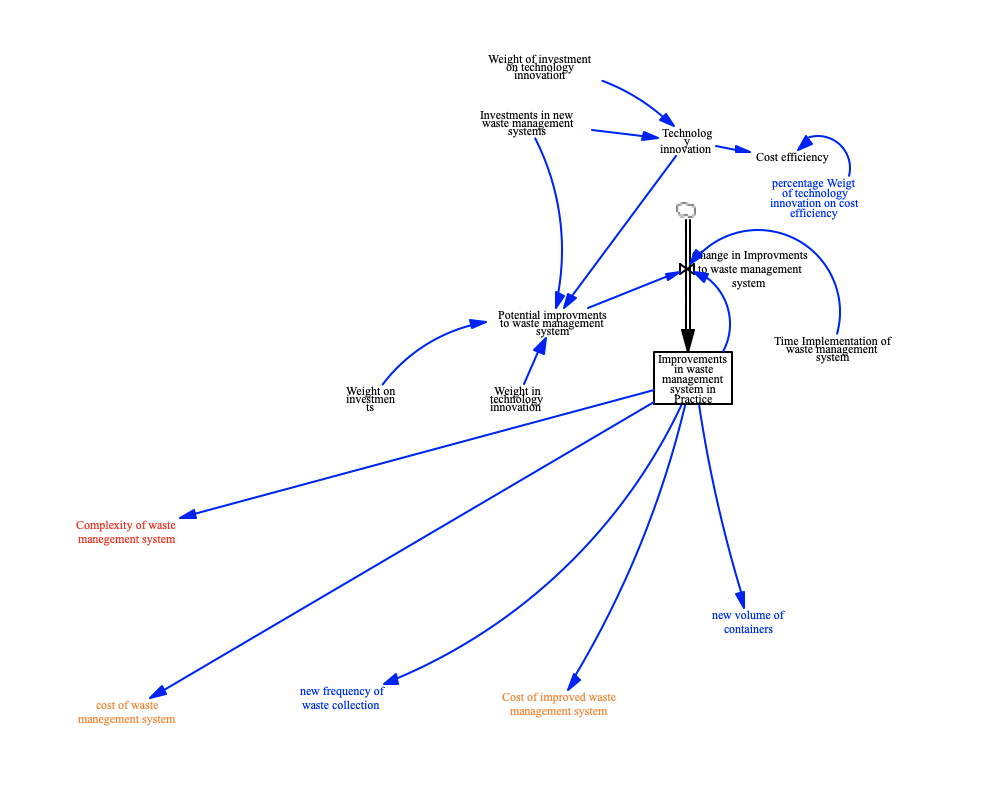
\includegraphics [scale=0.38,angle=360]{figures/improvementsystem.png}
\caption{Improvements System}
\label{fig:improvementsystem}
\end{figure}

\begin{flalign}
&\textbf{Technology innovation} =  &&  \text{[Dimensionless]}\nonumber\\
&I \times W && \nonumber
\end{flalign} 
\textit{Where:
\begin{itemize}
    \item[] $I$ =  Investments in new waste management systems
    \item[] $W$ = Weight of investments on technology innovation
\end{itemize}
}
\indent \newline
The endogenous variable technology innovation is dependent on the number of investments multiplied with how much of the new investments that leads to technological innovations. 

\begin{flalign}
&\textbf{Cost efficiency} =  &&  \text{[Dimensionless]}\nonumber\\
&TI \times W && \nonumber
\end{flalign} 
\textit{Where:
\begin{itemize}
    \item[] $TI$ = Technology innovation
    \item[] $W$ = Percentage weight of technology innovation on cost efficiency
\end{itemize}
}
\indent \newline
Cost efficiency is dependent on the weight of technology innovation which reduces the waste management system costs.

\begin{flalign}
&\scriptstyle\textbf{Percentage weight of technology innovation on cost efficiency} = 0.2 && \nonumber \text{[Dimensionless]}
\end{flalign} 
\indent \newline
The model assumes that 20 percent of technology innovation relates to improving cost efficiency. 

\begin{flalign}
&\textbf{Costs of waste management system} = && \text{[Dimensionless]}\nonumber\\
&1 + \frac{- PV \times WV + PF \times WF + PQ \times WQ - CE \times WC} {WV + WF + WQ - WC} && \nonumber
\end{flalign}
\textit{Where:
\begin{itemize}
    \item[] $PV$ = Procentual change in volume of containers
    \item[] $WV$ = Weight of volume on costs
    \item[] $PF$ = Procentual change in frequency of waste collection
	\item[] $WF$ = Weight of frequency on costs
	\item[] $PQ$ = Procentual change in quality of collected waste
	\item[] $WQ$ = Weight of quality on costs
	\item[] $CE$ = Cost efficiency
	\item[] $WC$ = Weight of cost efficiency
\end{itemize}
}
\indent \newline
Costs of the waste management system estimates a weighted average of the procentual change in volume of containers, frequency of waste collection, quality of collected waste and cost efficiency. The procentual change in volume of containers and cost efficiency reduce the costs, while the two other initiatives increase the costs. 

\begin{flalign}
&\textbf{Potential improvements to waste management system}= && \text{[Dimensionless]}\nonumber\\
&1 + \frac{I \times WI + TI \times WT} {WI +WT} && \nonumber
\end{flalign} 
\textit{Where:
\begin{itemize}
    \item[] $I$ = Investments in new waste management system
    \item[] $WI$ = Weight on investments
    \item[] $TI$ = Technology innovation
	\item[] $WT$ = Weight on technology innovation
\end{itemize}
}
\indent \newline
The model assumes that the potential improvements to the waste management system is dependent on a weighted average of investments and technology innovation.

\begin{flalign}
&\scriptstyle\textbf{Change in improvements to waste management system}= && \text{[Dimensionless/Year]}\nonumber\\
&\scriptstyle\frac{PI - I} {TI} && \nonumber
\end{flalign} 
\textit{Where:
\begin{itemize}
    \item[] $PI$ = Potential improvements to waste management system
    \item[] $I$ = Improvements in waste management system in practice
    \item[] $TI$ = Time implementation of waste management system
\end{itemize}
}
\indent \newline
The change in improvements to the waste management system is an inflow that estimates the change in improvements in the waste management system per year. 

\begin{flalign}
&\scriptstyle\textbf{Improvements in waste management system in practice}=&& \text{[Dimensionless]}\nonumber\\
&\scriptstyle\int_{0}^{t} \text{Change in improvements to waste management system} \times dt && \nonumber
\end{flalign}
\indent \newline
Improvements in waste management system in practice calculates the level of the improvements. The stock is influenced by the inflow change in improvements to waste management system.

\begin{flalign}
&\textbf{Costs of improved waste management system}=&& \text{[Dimensionless]}\nonumber\\
&\text{Improvements in waste management system in practice} && \nonumber
\end{flalign}
\indent \newline
Costs of improved waste management system is dependent on improvements in waste management system in practice. The variable represents the added costs from the improvements. 

\begin{flalign}
&\textbf{Complexity of waste management system}=&& \text{[Dimensionless]}\nonumber\\
&1 + \frac{- PV \times WV - PF \times WF + PQ \times WQ - (WI \times I - 1)} {WV + WF + WQ + WI} && \nonumber
\end{flalign} 
\textit{Where:
\begin{itemize}
    \item[] $PV$ = Procentual change in volume of containers
    \item[] $WV$ = Weight of volume on complexity
    \item[] $PF$ = Procentual change in frequency of waste collection
	\item[] $WF$ = Weight of frequency on complexity
	\item[] $PQ$ = Procentual change in quality of collected waste
	\item[] $WQ$ = Weight of quality on complexity
	\item[] $I$ = Improvements in waste management system in practice
	\item[] $WI$ = Weight of improvements in waste management system on complexity
\end{itemize}
}
\indent \newline
The complexity of waste management system is dependent on a weighted average of the procentual change in volume of containers, frequency of waste collection, quality of collected waste and improvements in waste management system in practice. The procentual change in volume of containers, frequency of waste collection and improvements in waste management system in practice reduces complexity, while the procentual change in quality of collected waste increases the complexity.

\begin{flalign}
&\textbf{New volume of containers}= && \text{[Dimensionless]}\nonumber\\
&\text{IF THEN ELSE}(I > 2, 1 - (PV \times I - 1), 1) && \nonumber
\end{flalign} 
\textit{Where:
\begin{itemize}
    \item[] $I$ = Improvements in waste management system in practice
    \item[] $PV$ = Percentage change in volume from new investment
\end{itemize}
}
\indent \newline
The new volume of containers is an IF THEN ELSE function, which is calculated in the following way; if improvements in waste management system in practice is larger than two, we estimate the procentual change in volume in containers from new investment. If improvements in waste management systems in practice is smaller or equal to two, the new volume of containers is unchanged. 

\begin{flalign}
&\textbf{New frequency of waste collection}= && \text{[Dimensionless]}\nonumber\\
&\text{IF THEN ELSE}(I > 2, 1 - ((I - 1) \times WI), 1) && \nonumber
\end{flalign} 
\textit{Where:
\begin{itemize}
    \item[] $I$ = Improvements in waste management system in practice
    \item[] $WI$ = Weight of improvements on frequency
\end{itemize}
}
\indent \newline
The new frequency of waste collection is calculated through an IF THEN ELSE function. If improvements in waste management system in practice is greater than two, the model computes improvements in waste management system in practice - 1, which is multiplied with the weight of improvements on frequency. If waste management system in practice is less than or equal to two, the new frequency of waste collection is unchanged.  

\subsection{Advertising System}

\begin{figure}[H]
\centering
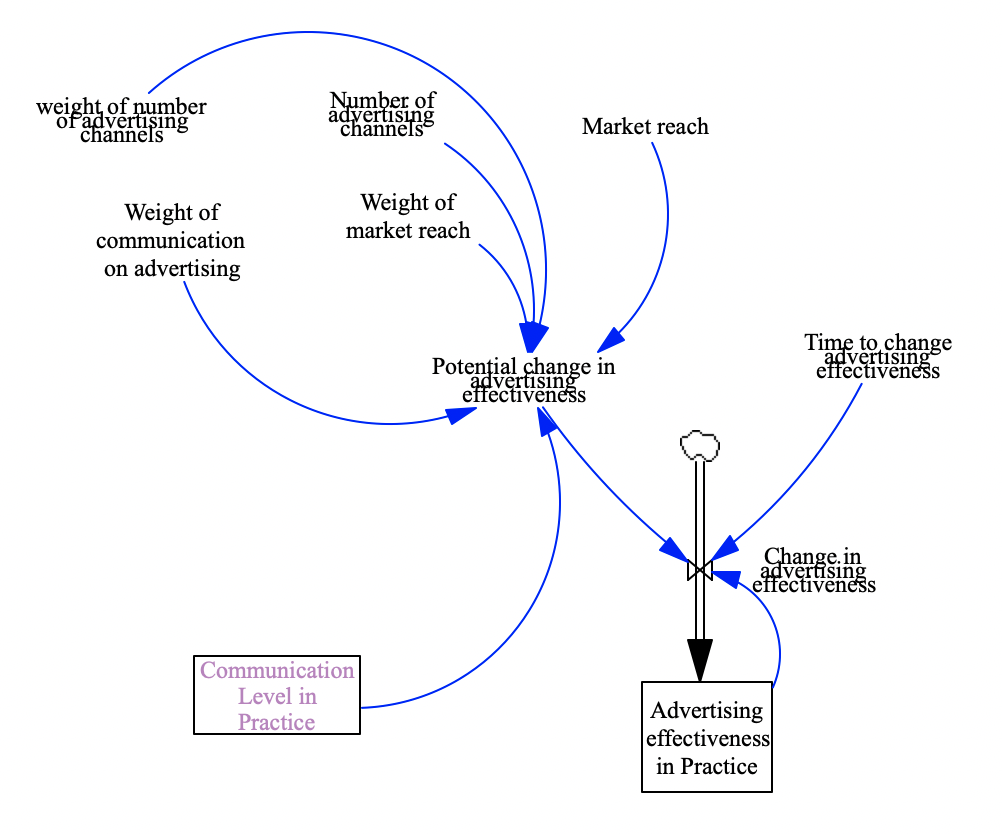
\includegraphics [scale=0.28,angle=360]{figures/advertisingsystem.png}
\caption{Advertising System}
\label{fig:advertisingsystem}
\end{figure}

\begin{flalign}
&\textbf{Communication level in practice}=&& \text{[Dimensionless]}\nonumber\\
&\int_{0}^{t}\text{Change of communication to citizens} \times dt && \nonumber
\end{flalign}
\indent \newline
The model assumes that the communication level in practice comes from changes in communication to citizens.

\begin{flalign}
&\textbf{Potential change in advertising effectiveness}=&& \text{[Dimensionless]}\nonumber\\
&1 + \frac{ C \times WC - 1 + A \times WA + M \times WM}  {WC + WA + WM} && \nonumber
\end{flalign} 
\textit{Where:
\begin{itemize}
    \item[] $C$ = Communication level in practice
    \item[] $WC$ = Weight of communication on advertising
    \item[] $A$ = Number of advertising channels
	\item[] $WA$ = Weight of number of advertising channels
	\item[] $M$ = Market reach
	\item[] $WM$ = Weight of market reach
\end{itemize}
}
\indent \newline
The potential change in advertising effectiveness is a weighted average of communication level in practice, the number of advertising channels, advertisements market reach and how they are weighted. This computes the level of advertising effectiveness per year.

\begin{flalign}
&\textbf{Time to change advertising effectiveness}= 4 && \text{[Year]}\nonumber\\
\nonumber
\end{flalign}
\indent \newline
The model assumes that the average time for advertising to be effective is four years.

\begin{flalign}
&\textbf{Change in advertising effectiveness}= && \text{[Dimensionless/Year]}\nonumber\\
&\frac{PA - A} {TA} && \nonumber
\end{flalign} 
\textit{Where:
\begin{itemize}
    \item[] $PA$ = Potential change in advertising effectiveness
    \item[] $A$ = Advertising effectiveness in practice
    \item[] $TA$ = Time to change advertising effectiveness
\end{itemize}
}
\indent \newline
The change in advertising effectiveness determines how effective the advertising has been per year. 

\begin{flalign}
&\textbf{Advertising effectiveness in practice}= && \text{[Dimensionless]}\nonumber\\
&\int_{0}^{t} \text{Change in advertising effectiveness} \times dt && \nonumber
\end{flalign}
\indent \newline
Advertising effectiveness in practice reports how effective the advertising campaign has been. The stock is influenced by the inflow change in advertising effectiveness. 

\subsection{Knowledge, Social Pressure, Attitude \& Behavior System}

\begin{figure}[H]
\centering
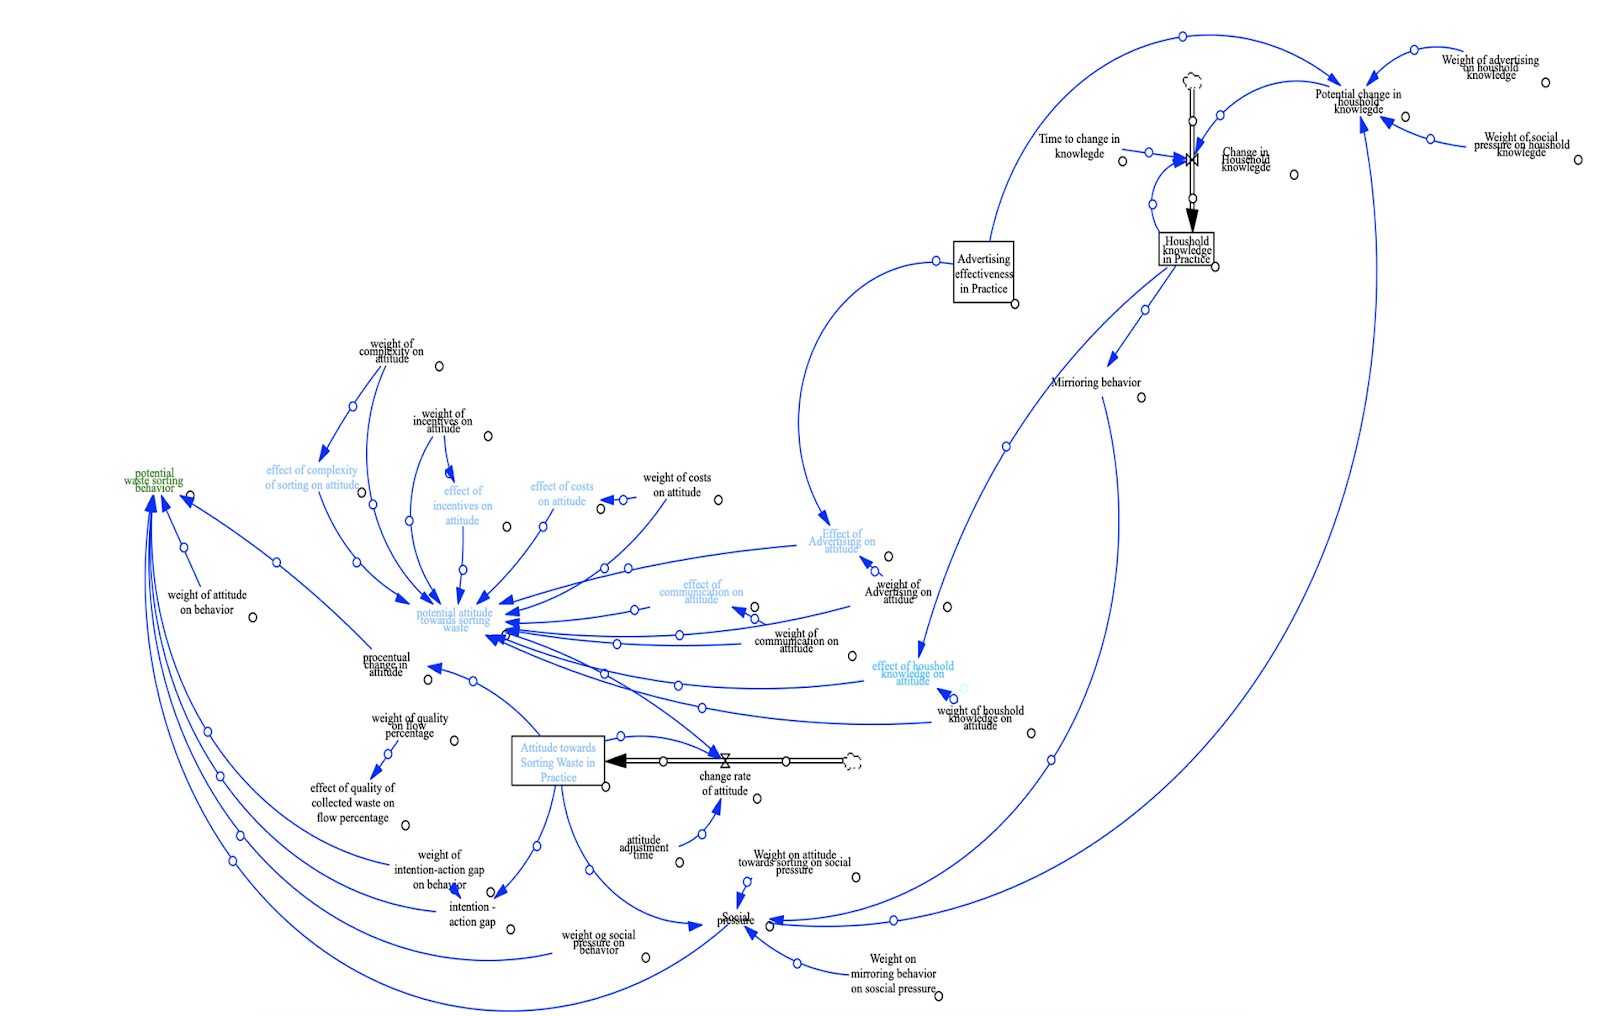
\includegraphics [scale=0.22,angle=360]{figures/lastsystem.png}
\caption{Knowledge, Social Pressure, Attitude \& Behavior}
\label{fig:lastsystem}
\end{figure}

\begin{flalign}
&\textbf{Potential change in household knowledge}= && \text{[Dimensionless]}\nonumber\\
&1 + \frac{ A \times WA - 1 + S \times WS}  {WA + WS} && \nonumber
\end{flalign} 
\textit{Where:
\begin{itemize}
    \item[] $A$ = Advertising effectiveness in Practice
    \item[] $WA$ =Weight of advertising on household knowledge
    \item[] $S$ = Social pressure
	\item[] $WS$ = Weight of social pressure on household knowledge
\end{itemize}
}
\indent \newline
The potential change in household knowledge is a weighted average of advertising effectiveness in practice, social pressures and how they are weighted. This shows how much advertising and social pressure change the knowledge of the households.  

\begin{flalign}
&\textbf{Time to change household knowledge} = 4 && \nonumber \text{[Year]}
\end{flalign} 
\indent \newline
The model assumes that it takes four years to achieve a change in household knowledge.

\begin{flalign}
&\textbf{Change in household knowledge}= && \text{[Dimensionless/Year]}\nonumber\\
&\frac{PH - H} {TH} && \nonumber
\end{flalign} 
\textit{Where:
\begin{itemize}
    \item[] $PH$ = Potential change in household knowledge
    \item[] $H$ = Household knowledge in practice
    \item[] $TH$ = Time to change household knowledge
\end{itemize}
}
\indent \newline
The change in household knowledge determines how effective advertising and social pressure has been on household knowledge per year.

\begin{flalign}
&\textbf{Household knowledge in practice}=&& \text{[Dimensionless]}\nonumber\\
&\int_{0}^{t}\text{Change in household knowledge} \times dt && \nonumber
\end{flalign}
\indent \newline
Household knowledge in practice reports the amount of knowledge the households have each year. The stock is influenced by the inflow change in household knowledge. 

\begin{flalign}
&\textbf{Weight of attitude towards sorting on social pressure} = 2 && \nonumber \text{[Dimensionless]}
\end{flalign} 
\indent \newline
The weight of attitude towards sorting on social pressure demonstrates the effect of attitude on social pressure. We conclude that attitude has a great influence on social pressure.

\begin{flalign}
&\textbf{Weight of advertising on household knowledge} = 3 && \nonumber \text{[Dimensionless]}
\end{flalign} 
\indent \newline
The weight of advertising on household knowledge determines how effective advertising is on household knowledge. We assume that advertising has a considerably larger impact on household knowledge than social pressure, since the target group utilizes substantial time on social media. 

\begin{flalign}
&\scriptstyle\textbf{Percentage of household knowledge who mirror behavior} = 0.1 && \nonumber \text{[Dimensionless]}
\end{flalign} 
\indent \newline
We assume that 10 percent of the target group mirrors others behavior towards waste sorting.

\begin{flalign}
&\textbf{Mirroring behaviour} = && \text{[Dimensionless]} \nonumber\\
&(H - 1) \times WH && \nonumber
\end{flalign} 
\textit{Where:
\begin{itemize}
    \item[] $H$ = Household knowledge in practice
    \item[] $WH$ = Weight of household knowledge on mirroring behavior
\end{itemize}
}
\indent \newline
Mirroring behavior is defined by household knowledge in practice multiplied with the weight of household knowledge. The function estimates how many with knowledge about waste sorting who can use mirroring to impact others.

\begin{flalign}
&\textbf{Social pressure}= && \text{[Dimensionless]} \nonumber\\
&1 + \frac{ A \times WA - 1 + M \times WM}  {WA + WM} && \nonumber 
\end{flalign} 
\textit{Where:
\begin{itemize}
    \item[] $A$ = Attitude towards sorting waste in practice
    \item[] $WA$ =Weight of attitude towards sorting on social pressure
    \item[] $M$ = Mirroring behavior
	\item[] $WM$ = Weight of mirroring behavior on social pressure
\end{itemize}
}
\indent \newline
Social pressure is a weighted average of attitude towards sorting waste in practice, mirroring behavior and how they are weighted. This computes the level of social pressure towards waste sorting. 

\begin{flalign}
&\textbf{Weight of advertising on attitude} = 3 && \nonumber \text{[Dimensionless]}
\end{flalign} 
\indent \newline
The weight of advertising on attitude determines how effective advertising is on attitude. We believe that advertising has a crucial effect on attitude due to our target group spending substantial time on social media.

\begin{flalign}
&\textbf{Weight of incentives on attitude} = 3 && \nonumber \text{[Dimensionless]}
\end{flalign} 
\indent \newline
The weight of incentives on attitude computes the effect of economic incentives on attitude. We conclude that economic incentives have a central effect on attitude because monetary benefits motivate our target group to sort their waste.

\begin{flalign}
&\textbf{Potential attitude towards sorting waste}= && \text{[Dimensionless]} \nonumber\\
&1 + \frac{ I + COM + COST + COMPLEX + H + A}  {WI + WCOM + WCOMPLEX + WCOST + WH + WA} && \nonumber
\end{flalign} 
\textit{Where:
\begin{itemize}
    \item[] $I$ = Effect of incentives on attitude
    \item[] $COM$ = Effect of communication on attitude
    \item[] $COST$ = Effect of costs on attitude
	\item[] $COMPLEX$ = Effect of complexity of sorting on attitude
	\item[] $H$ = Effect of household knowledge on attitude
	\item[] $A$ = Effect of advertising on attitude
	\item[] $WI$ = Weight of incentives on attitude
	\item[] $WCOM$ = Weight of communication on attitude
	\item[] $WCOMPLEX$ = Weight of complexity on attitude
	\item[] $WCOST$ = Weight of costs on attitude
	\item[] $WH$ = Weight of household knowledge on attitude
	\item[] $WA$ = Weight of advertising on attitude
\end{itemize}
}
\indent \newline
The potential attitude towards sorting waste is a weighted average of incentives, communication, cost, complexity, household knowledge, advertising and how they are weighted. This estimates the level of potential attitude towards waste sorting and how the variables impact attitude. 

\begin{flalign}
&\textbf{Intention-action gap}= && \text{[Dimensionless]} \nonumber\\
&(A - 1) \times WI \times -1 && \nonumber 
\end{flalign} 
\textit{Where:
\begin{itemize}
    \item[] $A$ = Attitude towards sorting waste in practice
    \item[] $WI$ = Weight of intention-action gap on behavior
\end{itemize}
}
\indent \newline
The intention-action gap determines how many with a positive attitude towards waste sorting, who still does not sort their waste. 

\begin{flalign}
&\textbf{Potential waste sorting behavior}= && \text{[Dimensionless]} \nonumber\\
&\scriptstyle{1 + \frac{- PV \times WV + PF \times WF + PQ \times WQ + PA \times WA + IAG \times WIAG + SP \times WSP} {WV + WF + WQ + WA + WIAG + WSP}} && \nonumber 
\end{flalign} 
\textit{Where:
\begin{itemize}
    \item[] $PV$ = Procentual change in volume of containers
    \item[] $WV$ = Weight of volume on behavior
    \item[] $PF$ = Procentual change in frequency of waste collection
	\item[] $WF$ = Weight of frequency on behavior
	\item[] $PQ$ = Procentual change in quality of collected waste
	\item[] $WQ$ = Weight of quality on behavior
	\item[] $PA$ = Procentual change in attitude
	\item[] $WA$ =Weight of attitude on behavior
	\item[] $IAG$ ="Intention-action gap"
	\item[] $WIAG$ =Weight of "intention-action gap" on behavior
	\item[] $SP$ =Social pressure
	\item[] $WSP$ =Weight of social pressure on behavior
\end{itemize}
}
\indent \newline
Potential waste sorting behaviour is a weighted average of the volume of containers, frequency of waste collection, quality of collected waste, change in attitude, social pressure and the intention-action gap. This computes the level of waste sorting behavior each year. 

\begin{flalign}
&\textbf{Change in waste sorting behavior}= && \text{[Dimensionless/Year]}\nonumber\\
&\text{IF THEN ELSE}(T < 2020, 0, (PWSB - WSBP) / AT) && \nonumber
\end{flalign} 
\textit{Where:
\begin{itemize}
    \item[] $T$ = Time
    \item[] $PWSB$ = Potential waste sorting behavior 
    \item[] $WSBP$ = Waste sorting behavior in practice
    \item[] $AT$ = Adjustment time of behavior
\end{itemize}
}
\indent \newline
Change in waste sorting behavior is an IF THEN ELSE function that estimates if time is lower than 2020, the function is zero. If the function is higher than or equal to 2020, the model computes the change in waste sorting behavior per year. 

\begin{flalign}
&\textbf{Weight of attitude on behavior} = 3 && \nonumber \text{[Dimensionless]}
\end{flalign} 
\indent \newline
The weight of attitude on behavior displays how effective attitude is on behavior. We assume that attitude is a crucial factor in sorting behavior.

\begin{flalign}
&\textbf{Economic incentives}= && \text{[Dimensionless]}\nonumber\\
&\scriptstyle\text{IF THEN ELSE}(MB > 1, (CDI \times CWMS + MB \times WMB) / CDI + WMB,\nonumber\\ 
&\scriptstyle{CDI \times CWMS)} && \nonumber
\end{flalign} 
\textit{Where:
\begin{itemize}
    \item[] $MB$ = Monetary benefits
    \item[] $CDI$ = Complexity-dependent incentives 
    \item[] $CWMS$ = Complexity of waste management system
    \item[] $WMB$ = Weight on monetary benefits
\end{itemize}
}
\indent \newline
Economic incentives is an IF THEN ELSE function which is calculated in the following way; if monetary benefits are larger than one, a weighted average of complexity and monetary benefits is computed. If monetary benefits are smaller than or equal to one, the model computes complexity-dependent incentives multiplied with the complexity of the waste management system. 

\begin{flalign}
&\textbf{Weight of monetary benefits} = 2 && \nonumber \text{[Dimensionless]}
\end{flalign} 
\indent \newline
We believe the initiative monetary benefits has a central impact on economic incentives.

\begin{flalign}
&\textbf{Weight of frequency on behavior} = 2 && \nonumber \text{[Dimensionless]}
\end{flalign} 
\indent \newline
The weight of frequency on behavior displays how effective frequency is on behavior. We assume that frequency has a great impact on sorting behavior.

\begin{flalign}
&\textbf{Weight of volume on behavior} = 3 && \nonumber \text{[Dimensionless]}
\end{flalign} 
\indent \newline
The weight of volume on behavior reflects how effective the volume of containers is on the behavior of sorting waste. We conclude that volume has a great effect on waste sorting behavior.

\section{Overview}

\begin{figure}[H]
\centering
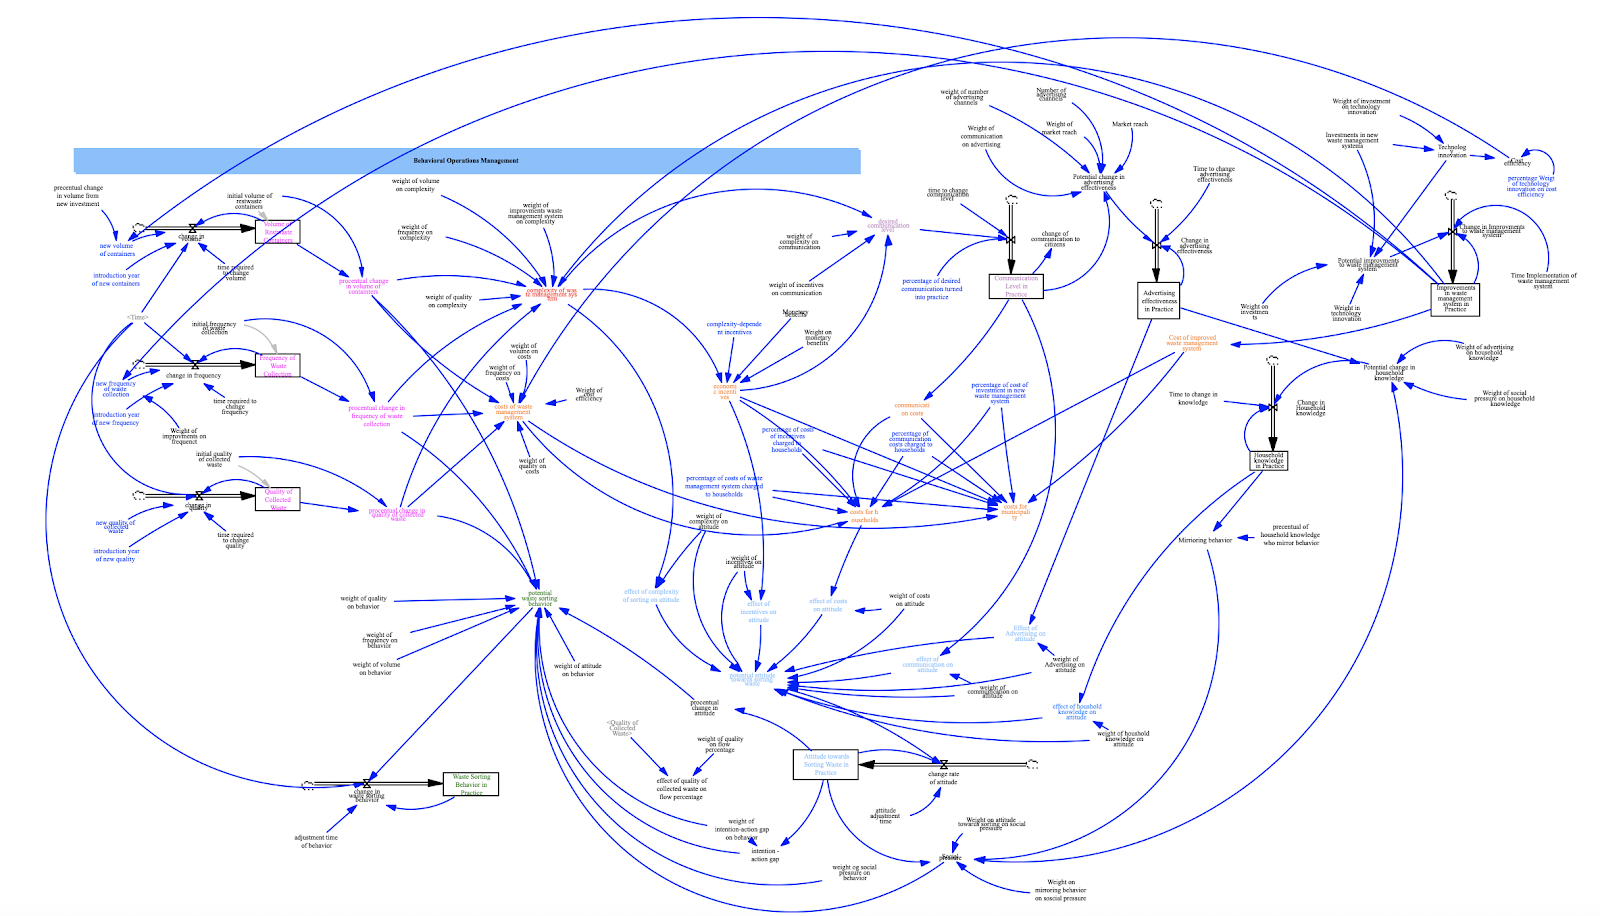
\includegraphics [scale=0.34,angle=90]{figures/overview.png}
\caption{Overview of The Stocks and Flows Model}
\label{fig:overview}
\end{figure}

\indent \newline
Figure 4.4 displays an overview of the complete stocks and flow model, regarding waste sorting behaviour. For further details, please see the attached Vensim file. 
